\newpage
\section{Анализ трафика}

С помощью GNS можно легко снимать дампы трафика. Для этого достаточно Wireshark

Для этого нужно сделать всего лишь следующее:
\begin{enumerate}
\item кликнуть правой кнопкой на линк между двумя устройствами
\item выбрать capture в контекстном меню
\item из меню справа выбрать нужное устройство и с помощью правой кнопки мыши выбрать Start Wireshark.
\end{enumerate}

В открывшемся окне Wiresharkа в реальном времени будут все пакеты которые отлавливаются на интерфейсе (рис. 10).

\begin{figure}[h!]
\centering
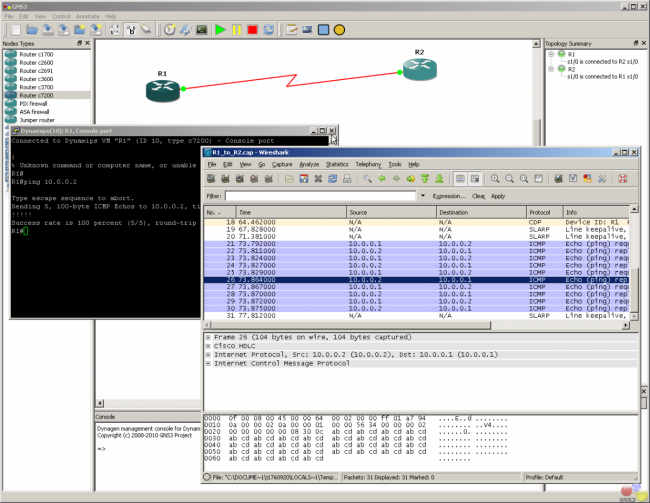
\includegraphics[scale=0.7]{res/pic010}
\caption{Дампы трафика с Wireshark}
\end{figure}